\chapter{Experiment 1: Noticeability of Distractors}\label{chap:ex1}
This chapter consists of the Method, Results and Discussion components for Experiment 1, which focuses on measuring detection thresholds for two different distracted states: walking and fighting. 

\section{Method}
Before delving into the deeper details of the methods that have been used for Experiment 1, it might be best to give a brief overview of the structure of it first. Experiment 1 consists of having participants play through the implemented Ensemble Retriever VR game, which is detailed in Chapter~\ref{chap:implementation}. As they play, the strength of rotation and curvature gains is gradually increased. Once the gains have reached a value that is high enough for the participant to notice, they have to press a button on their controller. This button press records a detection event for the relevant gain that has been applied. The strength of the detected gain is then decreased so it can rise again until the next time it is detected. After finishing, participants answer a short demographical post-test questionnaire with some optional qualitative feedback. 

The following sections detail the methods that have been employed to make this possible and what the focus of the measurements is. 

\subsection{Null Hypothesis}
When it comes to estimating detection thresholds, one interesting comparison would have been to see how different detection thresholds are between an undistracted and distracted state. While this would have been an interesting comparison, it does not necessarily fit all too well with the concept of fully integrating distractors into the experience. Since the distractors are such an important aspect of a game when integrated, it is not possible to remove them and retain the same experience. This tight coupling makes it challenging to compare distracted and undistracted conditions from a validity point of view as the experience would be significantly different without distractors. Instead, in order to keep the same experience for all participants, this experiment focuses on comparing two different distracted states. These two states consist of the walking state and the battle state in the game. 

While walking around in Ensemble Retriever, the player is distracted to some degree as the act of simply playing the game itself would be considered as an abstract distractor. There are some elements like the fireflies in the environment that could be considered as concrete distractors as well. Furthermore, there are a few other elements that contribute to an increased cognitive load and additional distraction in this state. These consist of the working memory task in the game (remembering the clues that fireflies provide), some basic path planning and being prepared to press the detection button as soon as the player notices any redirection. The battle state on the other hand, primarily distracts the player through the use of concrete distractors which consist of the distractor that the player has to fight as well as the projectiles that it fires. This state is also where most of the challenge in Ensemble Retriever lies as players need to figure out how to deal with the various projectile attacks and counterattack properly. 

By having these two interlinked states in the game that each participant takes part in, the experiment itself can be considered as using a within-subjects style of design. Given that the players move very little during battles, it is primarily rotation gain thresholds that are the most relevant to compare between these two states (curvature gains are only applied when walking). Since distraction/engagement is identified as a detection threshold variable in Chapter~\ref{chap:relatedWork}, it would thus be interesting to see what the differences in rotation gain thresholds are between the two states. As such, the following null hypothesis has been established:

\begin{description}
\item[$E_1H_0$: ] The mean detection thresholds for the battle state in Ensemble Retriever are not significantly wider than the walking state.
\end{description}

The expectation for the measurements is that that the larger amount of distraction that results from battles should in turn result in it becoming harder to notice redirection. 

\subsection{Estimating Detection Thresholds}\label{sec:ex1EstimationMethod}
In order to test the previously mentioned null hypothesis, it is first necessary to understand how the thresholds are estimated. As already mentioned in Section~\ref{sec:ethics}, the standard procedure for estimating detection thresholds has a high risk of cybersickness, which makes it unfeasible to use from an ethical point of view. The procedure can also be seen as incompatible with the concept of fully integrated distractors, meaning that a different approach is needed for this experiment.  

Instead, this experiment makes use of an alternative approach which is inspired by one of the experiments that Fuglestad performed in his redirected walking research~\cite{fuglestad2018redirected}: Incrementally increasing gains until they are noticed. This approach should minimise the risk of potential cybersickness as the possibility of reaching beyond the comfort/cybersickness threshold for individuals is lower. It should be noted that since the estimation method is different, it may of course not be as accurate as the standard procedure from Steinicke et al.'s research~\cite{5072212}. The use of estimation method should in this case be considered as a variable that may affect the estimated thresholds in addition to the previously mentioned variables in Table~\ref{table:DTVariables}.

\subsubsection{Incremental Gain Increases}
The incremental increase in gains is handled in two steps:

\begin{enumerate}
    \item Before each increment, a time step within the range of 2.5-7.5 seconds is randomly chosen. Once the duration of this chosen time step has expired, a random gain will be chosen for incrementing.
    \begin{itemize}
        \item It does not make sense to accumulate curvature gains when the user cannot experience them. As such, the potential options to increment vary somewhat depending on the state of the game:
        \item In the walking state: curvature, negative rotation and positive rotation gains are possible options.
        \item In the battle state: negative rotation and positive rotation gains are possible options.
    \end{itemize}
    \item Whenever a gain is incremented, it is done at a random amount within a given range:
    \begin{itemize}
        \item Rotation gains are incremented by $\pm2.5$-$7.5\%$ each increment. Only one type of rotation gain is incremented each time.
        \item Curvature radius is decreased by $2.5$-$7.5m$ each increment.
    \end{itemize}
\end{enumerate}
All of these random choices are handled through the use of a Mersenne Twister library~\cite{MersenneTwisterLibraryLink}. In this case, an SFMT implementation~\cite{saito2008simd} has been used to generate random integers corresponding to each choice. 

Once the experiment starts, all gains start at a default value. This default value is 0 for rotation gains and a 23m for the curvature gain radius. The reasoning for 23m as the default value for curvature radius is since Steinicke et al. initially found 22m as the threshold for curvature gains in their study~\cite{5072212}. Other studies have generally found lower values as the threshold, but 23m is set as the starting point as it is right above the highest estimated threshold by any studies seen in the literature sample for this thesis.

One potential issue that can arise with this type of method is that the participant does not move their head or body for some time. This results in an unnoticed accumulation of gains which might be uncomfortable and in the worst case result in cybersickness. To decrease the risk of large gain accumulation, a variety of caps have been introduced for each type of gain which cannot be exceeded:
\begin{itemize}
    \item Negative rotation gains cannot go lower than a value of -0.75. In this case, a gain of -1 would counteract any rotation on the y-axis and give the impression of this axis being frozen. If we use Steinicke et al.'s rotation gain semantics~\cite{5072212}, this would be the equivalent of a 0.25 multiplier. 
    \item Positive rotation gains cannot exceed a value of 1. This is the same as the strength that is applied when using the 2:1 Turn reset method. If we use Steinicke et al.'s rotation gain semantics~\cite{5072212}, this would be the equivalent of a 2.0 multiplier. 
    \item Curvature radius cannot go lower than a value of 2.5m. A radius of 1m is the lowest that the Redirected Walking Toolkit can use in this scenario.\todo{Somewhat weak justification maybe? As far as I know, no other research have identified curvature gain thresholds lower than about 3m. Steinicke et al. mentions \textasciitilde3.3 being noticeable, but usable for example(not a threshold per se)}. 
\end{itemize}

Given the usage of caps in the experiment, there may be several detections which reach these limits during certain situations. In these cases, capped detection values point towards the possibility of being able to further increase redirection, but that the gain has been capped to avoid possible increases in cybersickness.
   
\subsubsection{Detection Events}
Once the participant presses a button on their controller to signify that they notice they are being redirected, the following procedure takes place in the background:

\begin{itemize}
    \item The last 0.5 seconds of applied gains are always stored by the software.
    \item Once the detection button has been pressed, the gain that has had the largest prevalence in this buffer is chosen as the detected gain. 
    \item The detected gain is then halved for rotation gains or increased by 25\% for curvature radius as a means to ''reset'' while also allowing gains to quickly rise back towards the next detection event.
\end{itemize}

Already established methods like Steinicke et al.'s~\cite{5072212} make use of multiple buttons where the users for example can indicate whether they noticed that their head rotation was larger or lower than in reality. The reasoning for instead opting for a one button procedure is that it should be as simple as possible for the user to notify that they have detected something. In the case of standard estimation procedures, the entire focus of the participant is on the experiment itself, making multiple buttons feasible. In the case of this experiment though, the user is playing through a game and it would not be ideal to require additional mental processing when they already are engaged and focused on something else. Doing otherwise would detract from the point of using distractors as the focus of the user primarily should be on those. 

\subsection{Performance Data Collection}
As the participants play through Ensemble Retriever, the software itself collects a large variety of analytical data per frame. The general thought process behind recording data every frame is to provide insight into the whole runtime of the experiment and allow for deeper analysis if necessary around detection events. This data collection consists of data like the strength of gains at any given frame, whether a distractor was active, which distractor was active, whether a gain was detected and so on. The full list and a description for each piece of data that is collected can be found in Section~\ref{sec:ex1dataformat} as it is too long to reasonably mention in this section.

\subsection{Participant Sample}
This section consists of information on how the acquired participants were sampled, an overview of the demographics in the sample, what information participants were given and miscellaneous information. 

\subsubsection{Sampling Procedure}
The sampling procedure for this experiment consisted of the following methods:

\begin{enumerate}
    \item The experiment was advertised by supervisors during lectures.
    \item Posters advertising for the experiment were posted around campus.
    \item Advertisement on the local NTNU. Discord\footnote{\url{https://discordapp.com/}} server.
    \item Convenience Sampling.
\end{enumerate}

Participants were given access to a doodle poll\footnote{\url{https://doodle.com/}} where they could choose between a variety of time slots for when they wanted to partake in the experiment. Participants made use of aliases for this sign-up process. As compensation for participating, all participants received some chocolate. In total, 22 participants took part in Experiment 1. One of these includes the author of the thesis. 

\subsubsection{Sample Demographics}
In order to provide some demographics insights, participants were asked to answer a post-test questionnaire. The demographics questionnaire that participants answered can be found in Appendix~\ref{app:demographicsQuestionnaire}.

The sample itself primarily consisted of students within the age range of 18-24 years. 22 of the participants identified as male while 2 identified as female. Among the participants, only one needed to remove any optical corrections to use the HMD. In this participants' case, it should be noted that this was their preferred way to enjoy VR and did not negatively impact their vision. 

7/22 participants have had prior experience with projects using redirected walking. Finally, Figure~\ref{fig:ex1PriorVRExperience} shows a histogram over the Likert scale answers for the prior VR experience of participants. 

\begin{figure}[tbph]
    \centering
    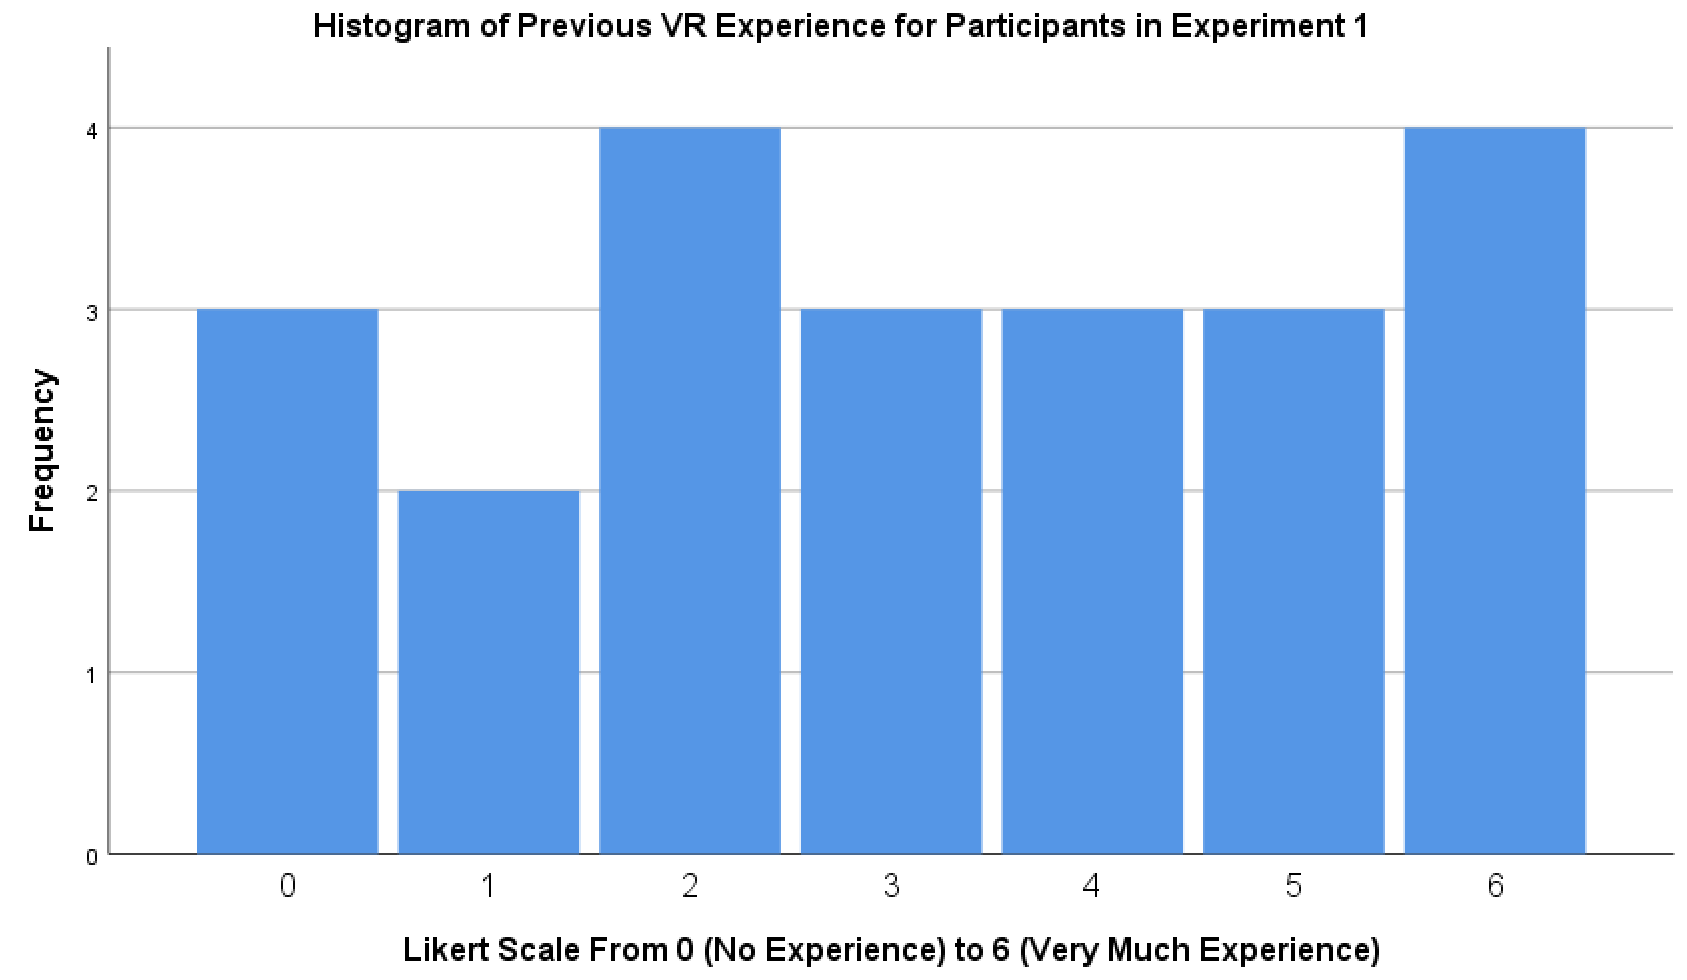
\includegraphics[width=0.75\textwidth]{figures/graphs/Experiment1VRExperienceHisto.png}
    \caption[Histogram on Prior VR Experience of Participants in Experiment 1]{This histogram shows the frequencies of what values participants provided in the demographics questionnaire of Experiment 1 in terms of prior VR experience.}
    \label{fig:ex1PriorVRExperience}
\end{figure}

\subsubsection{Information and Consent}
In terms of information and consent, participants were given an information and consent sheet where written consent was necessary. This information sheet was also available to read during the sign-up process. The information/consent sheets can be found in Appendix~\ref{app:informationconsent} for additional details. Furthermore, participants were also given some oral information before playing through Ensemble Retriever. This information can be summarised as follows:

\begin{itemize}
    \item A very brief summary of what redirected walking is was given if necessary.
    \item If the participant experienced any form of cybersickness at any point they were instructed to mention this so that the experiment could be stopped.
    \item Participants were encouraged to not walk too quickly for their own safety's sake.
    \item Participants were informed that the room tracking might fail for the controllers at times. If so, they need to wiggle it in the air for the problem to resolve.
    \item Participants were told they should be mindful of the tethered cable.
    \item Participants were told that they should not move too much around during battles to avoid potentially moving into walls. 
    \item Finally, participants were recommended to always keep a finger on the detection button so they could press it as soon as they noticed any redirection.
\end{itemize}

The specific details and wording that was used for this information can be found in Section~\ref{sec:ex1information}.

\subsubsection{Cancellation, Interruptions and Miscellaneous Information}
One of the participants had to cancel the experiment due to cybersickness. It should be noted that this participant mentioned they could easily get motion sickness which cybersickness can be considered a form of~\cite{mousavi2013review}. As such, it likely had some effect on why this was the only participant needing to cancel the experiment. This participant also mentioned that they mistakenly pressed the detection button several times. Due to this, they have been excluded from the sample, resulting in a sample of 21 participants. 

Two participants in the experiment did not manage to fully finish Ensemble Retriever due to the following reasons:
\begin{enumerate}
    \item One participant got interrupted by a fire drill towards the end of the game.
    \item One participant managed to disconnect the cables between the HTC Vive Linkbox and HMD towards the end of the game.
\end{enumerate}

The data for these two participants is still included in the sample as the interrupting moments happened late into the experiment. 

Finally, four participants did not provide any detection data at all. Two of these did not provide any detections as they did not notice being redirected. These were participants with no prior VR experience and as such, they mentioned that they had no prior reference points to use for detecting any unusual manipulations. The other two appear to have misunderstood which button to press on their controllers for detection despite the tutorial clearly labelling and showing which one to use. 

\subsection{Experiment Environment/Physical Space}\label{sec:ex1physicalRoom}
\begin{figure}[tbph]
    \centering
    \includegraphics[width=1\textwidth]{figures/images/roomLighthouses.png}
    \caption[Image of Experiment Environment]{These two images show a rough outline of the physical tracking space that was used with green lines. Red circles are used to outline the location of the Vive Lighthouses.}
    \label{fig:ex1room}
\end{figure}

\begin{figure}[tbph]
    \centering
    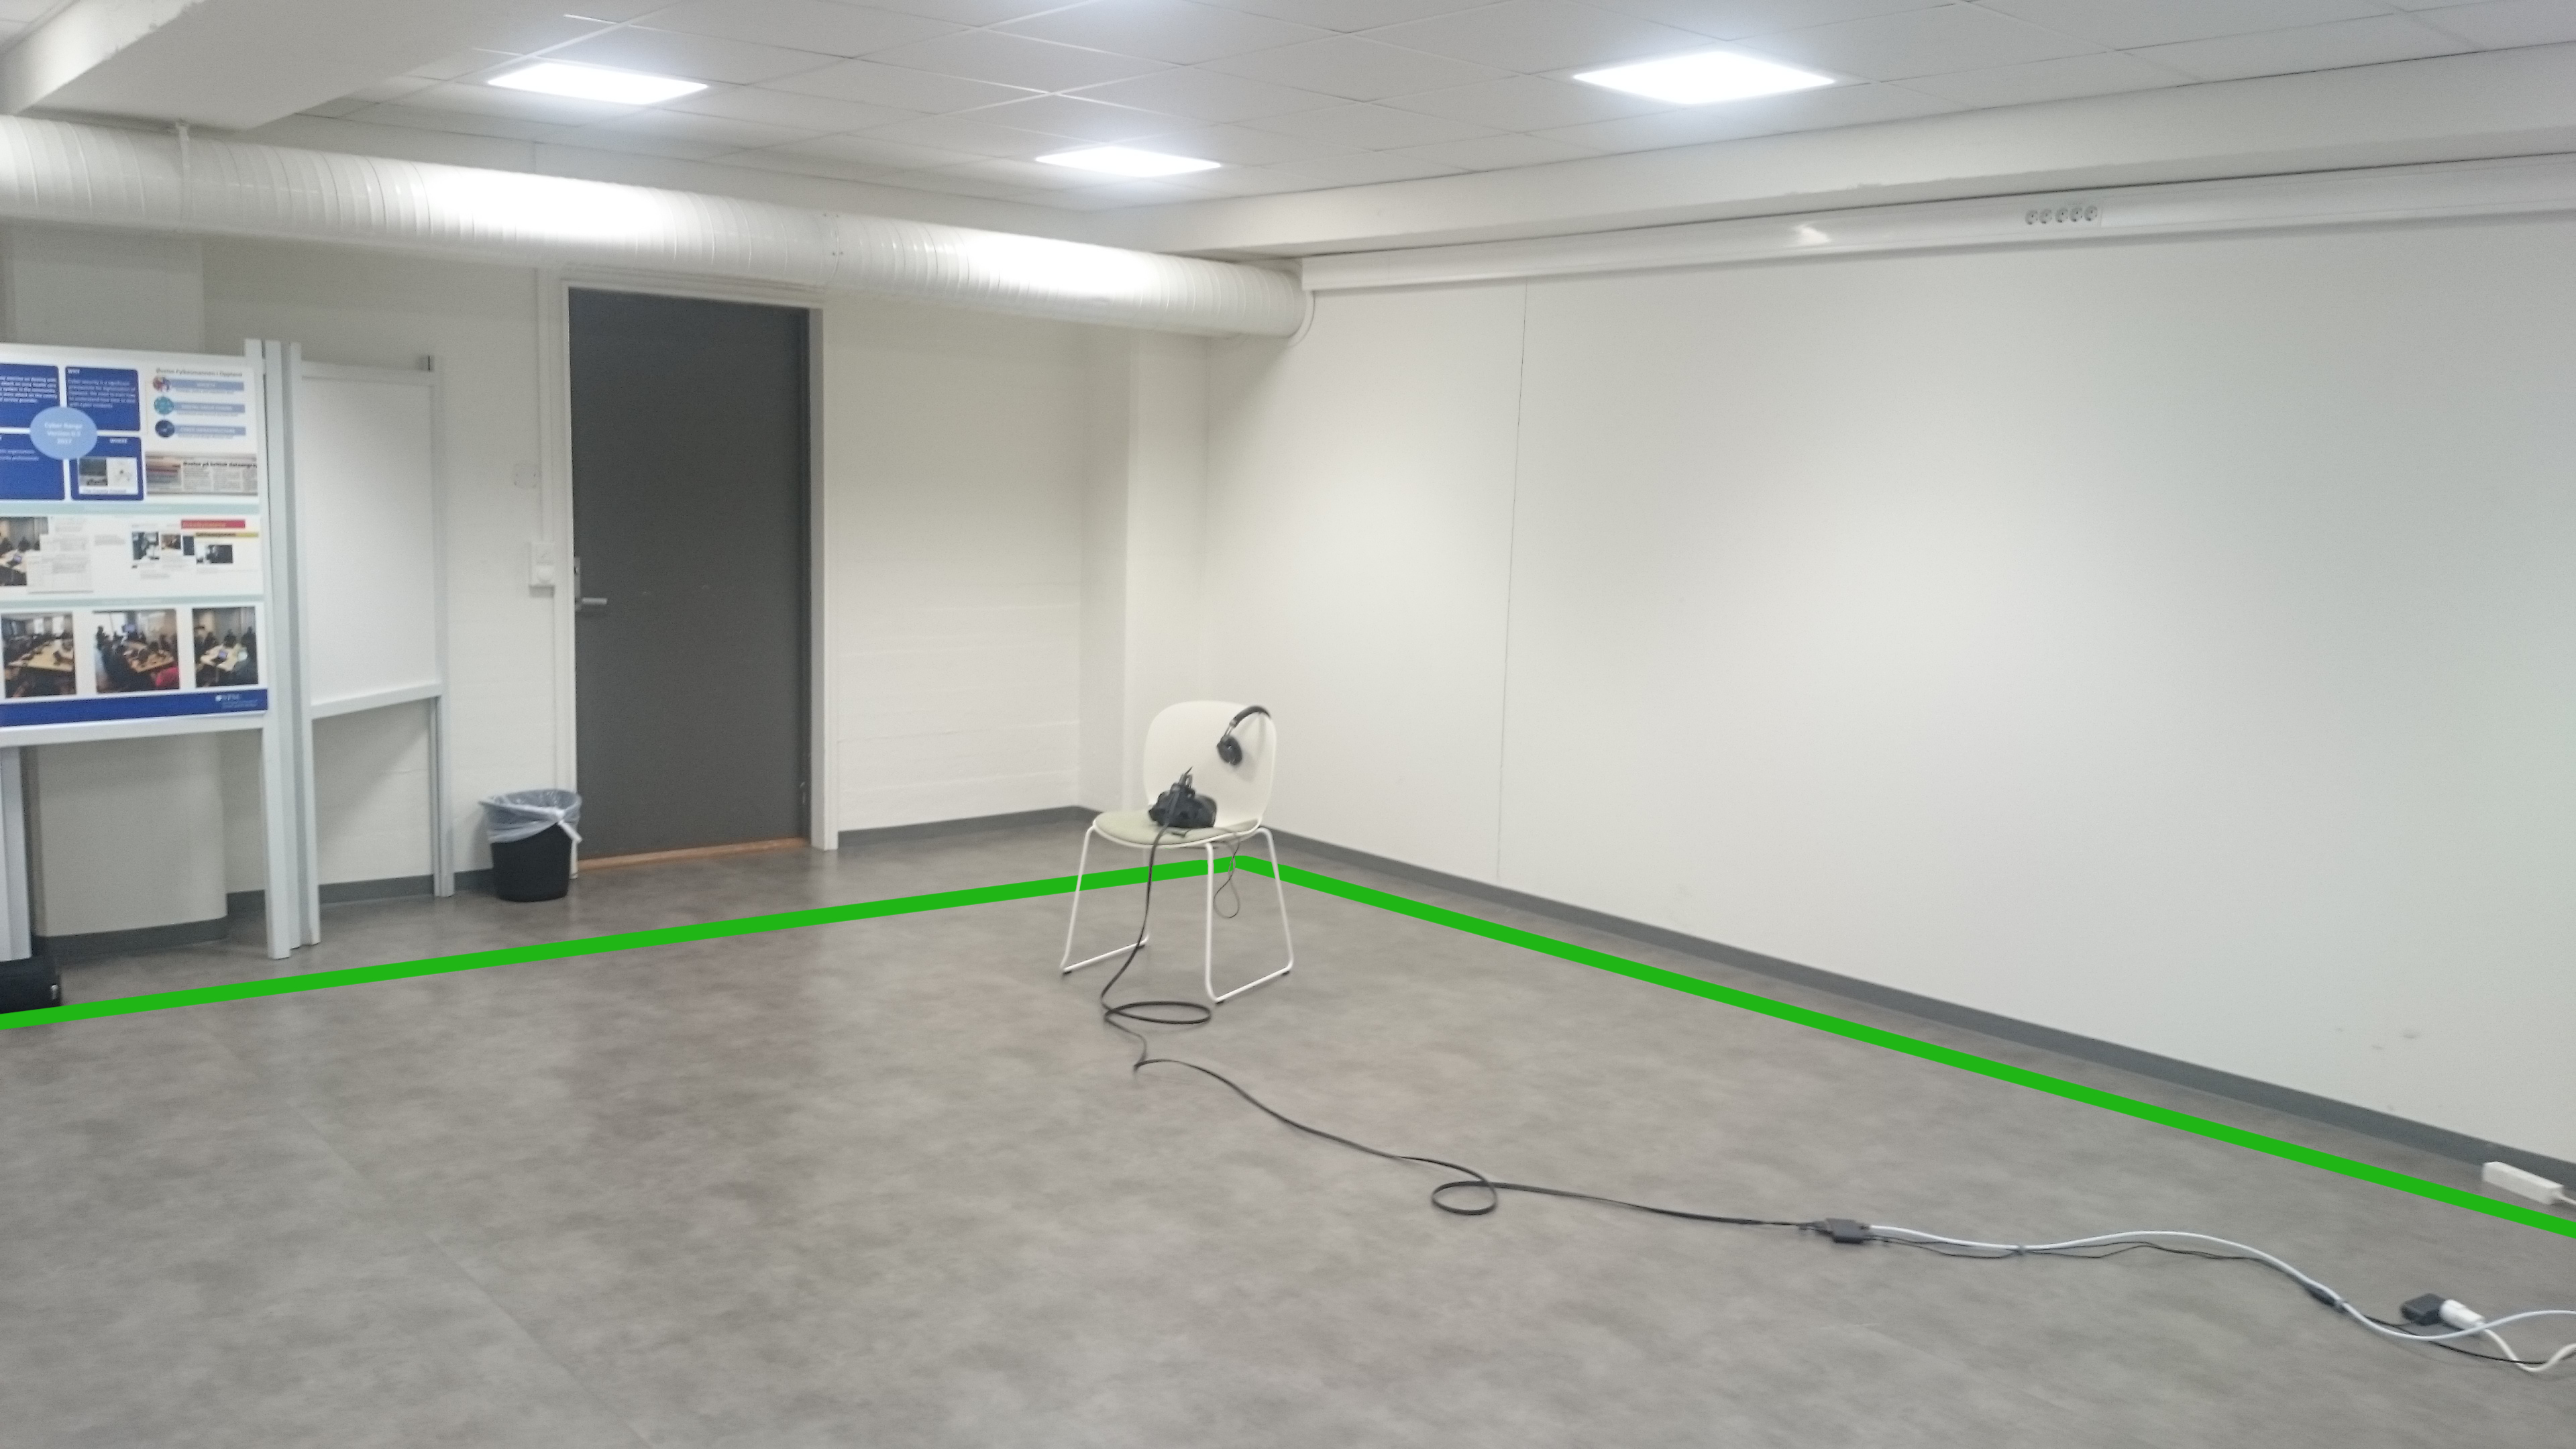
\includegraphics[width=1\textwidth]{figures/images/extraRoomImage.jpg}
    \caption[Supplementary Image of Experiment Environment]{This supplementary image shows more of the physical tracking space.}
    \label{fig:ex1roomImage2}
\end{figure}

\begin{figure}[tbph]
    \centering
    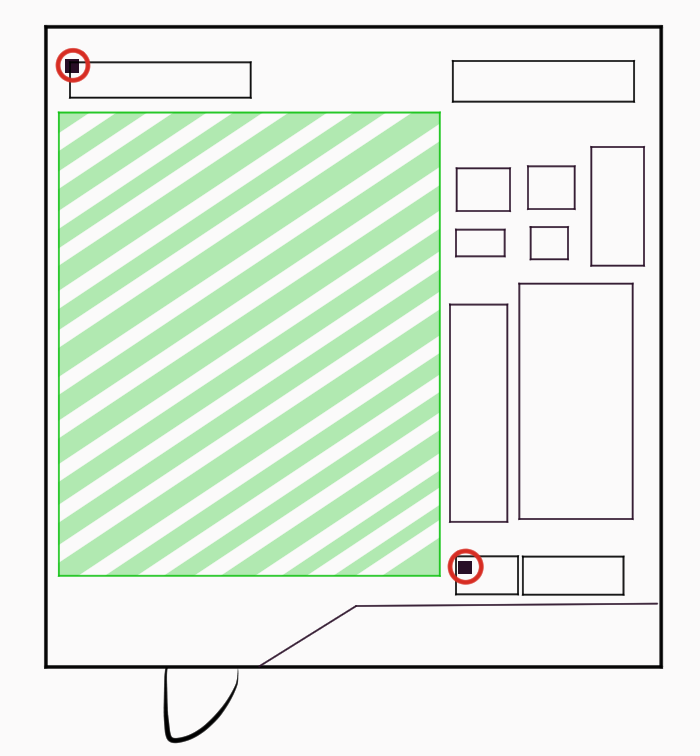
\includegraphics[width=0.5\textwidth]{figures/images/topDownRoom.png}
    \caption[Top Down Representation of Experiment Environment]{This sketch represents roughly how the experiment room was used from a top down view. The green shaded area is the physical tracking space while the location of the Vive Lighthouses is signified with red circles.}
    \label{fig:ex1roomTopDown}
\end{figure}

The experiment itself took place in a room with a physical tracking space of approximately 5m x 5.75m and can be seen in Figure~\ref{fig:ex1room}, Figure~\ref{fig:ex1roomImage2} and Figure~\ref{fig:ex1roomTopDown}. The lights in the room were turned off during the experiment to prevent any potential reference points to the floor which might have been gleaned from under the HMD. Doing so is a relatively standard procedure as Steinicke et al. made use of this in their initial detection threshold experiment~\cite{5072212}. 

\subsection{Data Post Processing}\label{sec:ex1postprocessing}
In terms of rotation gain detections, it is not uncommon to find detections in the recorded data that have been set to a value of 0. There are four potential scenarios where this can happen:
\begin{enumerate}
    \item The player noticed a gain, but by the time they pressed the button they had already been aligned and gains were disabled.
    \item The player noticed that rotation gains were disabled after they had been aligned. 
    \item The player pressed the button thinking they had noticed a gain while they in reality did not experience any.
    \item The player pressed the button a bit late, during a time where their head did not move. This can create the assumption that not applying gains was the most prevalent in the 0.5-second buffer.  
\end{enumerate}

Among these four, it is primarily cases 1 and 4 that would be the most important to deal with as some additional processing around these could yield additional detection data. As such, a post-processing step was conducted to attempt retrieving the correct values for these cases. The details on how the post-processing was conducted can be found in Section~\ref{sec:ex1postprocessingdetails}. 

It should be noted that the post-processing step for the first 13 participants could only be partially conducted. The reasoning for this was due to a bug in the data recording that affected the validity of certain variables which were aimed to be used for post-processing. In particular, there was an issue where a set of ratio variables representing the ratios of gains applied in a specified time buffer before each detection was not recorded properly. As a result, the only post-processing that was possible for these participants was alternative 1 for case 1 which is described in Section~\ref{sec:ex1postprocessingdetails}. This bug was fixed for all subsequent participants and as such, the full post-processing was used for these. 


   
